\section{Introduction}\label{sec:introduction}

An instance of bin packing is an explicitly listed collection of rational
item sizes in $(0,1]$, encoded in binary. A bin may contain any
subcollection of total size at most one. Write $\OPT(I)$ for the minimum
number of bins needed to pack an instance $I$, and $a_i$ for the size of
its $i$th item copy. We consider deterministic
algorithms whose running time is polynomial in the length of this explicit
encoding. The additive approximation question asks whether one algorithm
and one absolute constant $C$ can guarantee at most $\OPT(I)+C$ bins for
every instance $I$.
Williamson and Shmoys included this constant-additive question among
the open problems in their 2011 book on approximation
algorithms~\cite[Chapter~17, Problem~3]{WilliamsonShmoys2011}.

The configuration linear program assigns nonnegative weights
to feasible bin patterns and minimizes their total weight subject to
covering the item demands. Its cutting-stock antecedents include
Eisemann's formulation and Gilmore and Gomory's column-generation
method~\cite[p.~849]{GilmoreGomory1961}.
We use the ordinary formulation in numerical
size types. We will also prove the same gap for the stronger formulation
whose patterns are subsets of the individual item copies.

\subsection{Configuration relaxations and integer rounding}

\begin{definition}[Configuration relaxations]\label{def:configuration-lp}
For the ordinary type formulation, let $\mathcal S$ be the set of
distinct numerical sizes and let $n_\sigma$ be the multiplicity of
$\sigma\in\mathcal S$.  Its configurations are all integer vectors
\[
 \mathcal C=\left\{(c_\sigma)_{\sigma\in\mathcal S}
       \in\Z_{\ge0}^{\mathcal S}:
       \sum_{\sigma\in\mathcal S}\sigma c_\sigma\le1\right\}.
\]
The Gilmore--Gomory relaxation is
\begin{equation}\label{eq:type-configuration-lp}
 \LP=
 \min\left\{\sum_{\mathbf c\in\mathcal C}z_{\mathbf c}:
       z_{\mathbf c}\ge0,\quad
       \sum_{\mathbf c\in\mathcal C}c_\sigma z_{\mathbf c}
          \ge n_\sigma\quad(\sigma\in\mathcal S)\right\}.
\end{equation}
In particular, type configurations may repeat a size; their
multiplicities are limited by capacity, rather than by the input
multiplicities.

Give the input items distinct physical indices in a set $\mathcal I$,
with size $a_i$ at index $i$, even when some sizes coincide.
An individual-copy configuration
is a subset $H\subseteq\mathcal I$ with $\sum_{i\in H}a_i\le1$.
Writing $\mathcal H$ for all such subsets, define
\begin{equation}\label{eq:individual-configuration-lp}
 \OPT_{\mathrm{LP,ind}}=
 \min\left\{\sum_{H\in\mathcal H}y_H:
       y_H\ge0,\quad
       \sum_{H\ni i}y_H\ge1\quad(i\in\mathcal I)\right\}.
\end{equation}
\end{definition}

Both programs are lower bounds on $\OPT(I)$. The distinction between
patterns that may repeat a size beyond its input multiplicity and patterns
limited by available copies is relevant to integer-rounding questions;
see Kartak, Ripatti, Scheithauer, and Kurz~\cite{KartakRipattiScheithauerKurz2015}.
Here $\LP(I)$ always denotes the unrestricted numerical-type formulation
in Equation~\eqref{eq:type-configuration-lp}. We prove its value and the
individual-copy value separately for our instances.

The integer round-up property asks whether the integral optimum equals
the fractional optimum rounded up. Marcotte studied this property for
cutting stock and exhibited an instance for which it
fails~\cite{Marcotte1985,Marcotte1986}. Scheithauer and Terno investigated
the modified bound~\cite{ScheithauerTerno1995,ScheithauerTerno1997}
\begin{equation}\label{eq:mirup}
  \OPT(I)\le \lceil\LP(I)\rceil+1,
\end{equation}
now known as the \emph{Modified Integer Round-Up Conjecture}.
The algorithmic question and this structural question require separate
arguments: Equation~\eqref{eq:mirup} concerns the existence of a packing,
whereas an approximation algorithm must construct one efficiently.

\subsection{Results}

Our first result is an unconditional family of gaps for both
configuration relaxations.

\begin{theorem}[Unbounded configuration gap]\label{thm:unbounded-gap}
For every integer $c\ge0$, there is a finite rational bin-packing instance
$I$ and an integer $B$ such that every item size exceeds $1/6$ and
\begin{equation}\label{eq:main-gap}
  \LP(I)=B,
  \qquad \OPT(I)>B+c.
\end{equation}
The equality for the fractional optimum also holds for the configuration
LP whose patterns are subsets of the individual item copies.
\end{theorem}

Taking $c=1$ contradicts Equation~\eqref{eq:mirup}, so
Theorem~\ref{thm:unbounded-gap} disproves the Modified Integer Round-Up
Conjecture. The integral LP value in the construction makes this a gap
beyond the conjectured rounding allowance, without any ambiguity caused
by the ceiling.

The same construction yields hardness for every fixed additive allowance.

\begin{theorem}[Constant-additive hardness]\label{thm:additive-hardness}
For every fixed integer $c\ge0$, it is NP-hard to distinguish pairs $(I,B)$
such that $I$ packs into $B$ bins from pairs such that $I$ cannot be packed
into $B+c$ bins.  Here $B$ is an integer supplied with the instance,
the item sizes are rational, and every item size is strictly greater
than $1/6$.
\end{theorem}

\begin{corollary}\label{cor:complexity-equiv}
A deterministic polynomial-time algorithm that always uses at most
$\OPT(I)+C$ bins for some absolute constant $C$ exists if and only if
$\classP=\classNP$.
\end{corollary}

Theorem~\ref{thm:unbounded-gap} assumes no separation of complexity
classes. Theorem~\ref{thm:additive-hardness} gives the conditional negative
answer to the algorithmic question through
Corollary~\ref{cor:complexity-equiv}. All constructions use sizes greater
than $1/6$, so each feasible bin contains at most five items.

\subsection{Approximation bounds and related constructions}

Fernandez de la Vega and Lueker used grouping of item sizes to obtain
an asymptotic approximation scheme~\cite{FernandezDeLaVegaLueker1981}:
for each fixed positive
$\varepsilon$, the multiplicative ratio can be made $1+\varepsilon$
once the optimum is sufficiently large. A fixed multiplicative excess
still allows an additive error that grows with the optimum.
Karmarkar and Karp combined grouping with approximate solution of
the configuration LP and repeated packing of its integral part,
obtaining an additive bound of order
$\log^2\OPT$~\cite{KarmarkarKarp1982}.
Rothvoss combined discrepancy-based rounding with grouping and gluing
of small items to improve this to order
$\log\OPT\log\log\OPT$~\cite{Rothvoss2013}.
Hoberg and Rothvoss first assembled items into containers and then
packed the containers into bins, obtaining order
$\log\OPT$~\cite{HobergRothvoss2017}.
The latter two algorithms are randomized, and their bounds hold relative
to the configuration LP.
These logarithmic upper bounds are compatible with
Theorem~\ref{thm:unbounded-gap}: the constructed instances can grow very
rapidly with the prescribed gap. We do not obtain a matching logarithmic
lower bound as a function of their size.

Earlier counterexamples and rounding obstructions explain two obstacles
to a larger gap. Caprara, Dell'Amico, D\'iaz-D\'iaz, Iori, and Rizzi
encoded edge-coloring obstructions in scalar bin sizes to produce
instances without the integer round-up
property~\cite{CapraraDellAmicoDiazDiazIoriRizzi2015}.
Such graph encodings provide a related way to transfer a combinatorial
obstruction into packing, but those examples do not establish unbounded
additive gaps. Newman, Neiman, and Nikolov, and Eisenbrand,
P\'alv\"olgyi, and Rothvoss used discrepancy constructions to prove
logarithmic obstructions for algorithms restricted to rounding a supplied
fractional support~\cite{NewmanNeimanNikolov2012,EisenbrandPalvolgyiRothvoss2013}.
An integral packing may use
other feasible configurations. A gap for the full configuration LP must
therefore control all such packings, rather than only the chosen support.
This is the task of our extraction argument.

The restriction to at most five items per bin does not fix the number of
distinct numerical sizes. Goemans and Rothvoss proved exact polynomial-time
solvability for a fixed number of sizes~\cite{GoemansRothvoss2014}, and
Koana and Kumabe have announced a fixed-parameter algorithm in that
parameter~\cite{KoanaKumabe2026}. These results concern a different
parameter regime. For subset-pattern formulations, the connection to
discrepancy of permutations yields bounds depending on the number of items
even when bin cardinality is fixed~\cite{EisenbrandPalvolgyiRothvoss2013};
the upper bounds for set covering with ordered replacement likewise
retain a logarithmic dependence on the number of items for fixed
cardinality~\cite{EisenbrandEtAl2011}.

\subsection{The graph-to-packing construction}

A vertex cover of a graph is a set of vertices containing at least one
endpoint of every edge. We prove a quantitative reduction from this
problem. For every fixed $c\ge0$ and $\rho>0$, an explicitly represented
graph with $n$ vertices and a cover target $k$ produces $5B$ items.
A cover of size at most $k$ gives a $B$-bin packing, while every packing
into at most $B+c$ bins gives a cover of size at most $k+\rho n$.
Theorem~\ref{thm:reduction} states the exact interface. The constants
depend on $c$ and $\rho$; for each fixed pair, the explicit list of items
and their binary encodings have polynomial length in the graph input.

\paragraph{Two interval families force a choice.}
For a chosen positive integer $d$, the first ingredient is a pair of
finite rooted trees with a quota at each positive depth.
Each tree separately has a marking that meets every
root-to-leaf path at least $d$ times while respecting these quotas.
When the same quotas are shared between both trees, however, the two
trees cannot both have every path marked even once.
Depth-constrained path hitting also occurs in the tree formulation of
resource minimization for fire containment~\cite{ChalermsookChuzhoy2010}.
We prove the particular two-tree property directly in
Lemma~\ref{lem:competing-trees}.

For each graph vertex we represent the two trees by nested interval
cells, with separate plus and minus regions. Cells at the same depth are
well separated. A local resource of a given length can cover points in
at most one cell at the corresponding depth; the number of such resources
is its depth quota. If every leaf cell requires $d$ units of coverage,
the competing-tree property forces almost $d$ additional, global resources
onto one of the two sides. The plus-side allocation will determine the
extracted vertex cover. Short test intervals for the incident edges are
placed beside the plus tree.

\paragraph{Five item roles encode interval coverage.}
An intended bin has a row item, an anchor item, a global auxiliary item,
a local auxiliary item, and a flag item. Rows, anchors, and local
auxiliaries carry graph-vertex labels. A row carries a baseline
coordinate $b$. In one kind of bin with equal labels, the auxiliary
lengths move it to a completion coordinate $h\le b$, and the anchor
supplies a deadline $z$.
The bin fits precisely when $h\le z$. Its half-open interval $[h,b)$
records the positions crossed by that move. Shifting $d$ deadlines from
the right endpoint of a test interval to its left endpoint forces $d$
additional completions at or before every point in that interval. Comparing
prefix counts turns this into a coverage requirement. The elementary
identity underlying this step is illustrated in
Figure~\ref{fig:interval-mechanism}.

\begin{figure}[htbp]
\centering
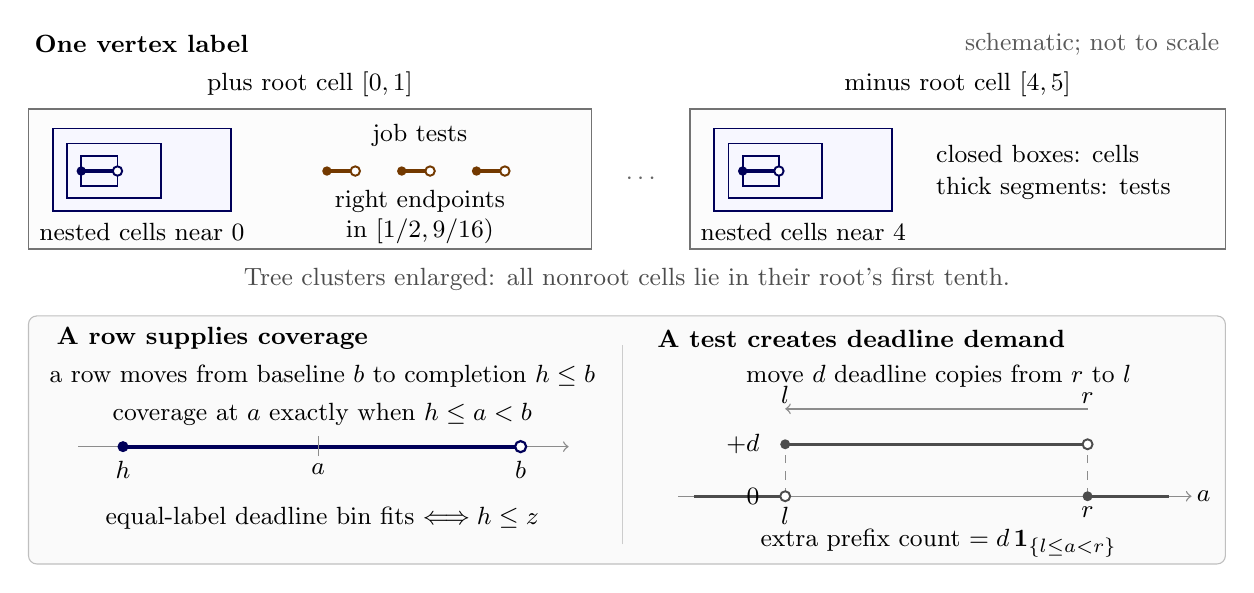
\begin{tikzpicture}[
  x=1cm,y=1cm,
  font=\fontsize{9.5}{11.5}\selectfont,
  every node/.style={inner sep=2pt},
  rootcell/.style={draw=black!55,line width=.6pt,fill=black!1},
  treecell/.style={draw=blue!35!black,line width=.65pt,fill=blue!3},
  test/.style={draw=blue!35!black,line width=1.5pt},
  jobtest/.style={draw=orange!45!black,line width=1.5pt},
  guide/.style={draw=black!45,line width=.5pt},
  heading/.style={font=\fontsize{9.5}{11.5}\selectfont\bfseries}
]
\node[heading,anchor=west] at (.15,6.65) {One vertex label};
\node[anchor=east,text=black!65] at (15.35,6.65)
  {schematic; not to scale};
\node at (3.725,6.14) {plus root cell $[0,1]$};
\node at (11.95,6.14) {minus root cell $[4,5]$};
\draw[rootcell] (.15,4.05) rectangle (7.30,5.83);
\draw[rootcell] (8.55,4.05) rectangle (15.35,5.83);
\node[text=black!60] at (7.925,4.94) {$\cdots$};

\foreach \offset in {0,8.40} {
  \begin{scope}[xshift=\offset cm]
    \draw[treecell] (.46,4.53) rectangle (2.72,5.58);
    \draw[treecell] (.64,4.70) rectangle (1.83,5.39);
    \draw[treecell] (.82,4.85) rectangle (1.28,5.23);
    \draw[test] (.82,5.04) -- (1.28,5.04);
    \fill[blue!35!black] (.82,5.04) circle (1.7pt);
    \draw[draw=blue!35!black,fill=white,line width=.7pt]
      (1.28,5.04) circle (1.7pt);
  \end{scope}
}
\node at (1.59,4.27) {nested cells near $0$};
\node at (9.99,4.27) {nested cells near $4$};
\node[align=left,anchor=west] at (11.60,5.02)
  {closed boxes: cells\\thick segments: tests};

\node at (5.12,5.50) {job tests};
\foreach \left/\right in {3.94/4.30,4.89/5.25,5.84/6.20} {
  \draw[jobtest] (\left,5.04) -- (\right,5.04);
  \fill[orange!45!black] (\left,5.04) circle (1.7pt);
  \draw[draw=orange!45!black,fill=white,line width=.7pt]
    (\right,5.04) circle (1.7pt);
}
\node at (5.12,4.66) {right endpoints};
\node at (5.12,4.27) {in $[1/2,9/16)$};
\node[text=black!70] at (7.75,3.67)
  {Tree clusters enlarged: all nonroot cells lie in their root's first tenth.};

\draw[draw=black!25,fill=black!2,rounded corners=3pt]
  (.15,.05) rectangle (15.35,3.20);
\node[heading,anchor=west] at (.43,2.91) {A row supplies coverage};
\node[heading,anchor=west] at (8.06,2.91) {A test creates deadline demand};
\draw[draw=black!20] (7.69,.30) -- (7.69,2.83);

\node at (3.88,2.43)
  {a row moves from baseline $b$ to completion $h\le b$};
\draw[guide,->] (.78,1.54) -- (7.01,1.54);
\draw[test] (1.35,1.54) -- (6.40,1.54);
\fill[blue!35!black] (1.35,1.54) circle (2pt);
\draw[draw=blue!35!black,fill=white,line width=.8pt]
  (6.40,1.54) circle (2pt);
\draw[guide] (3.83,1.42) -- (3.83,1.67);
\node[anchor=north] at (1.35,1.43) {$h$};
\node[anchor=north] at (3.83,1.40) {$a$};
\node[anchor=north] at (6.40,1.43) {$b$};
\node at (3.88,1.95) {coverage at $a$ exactly when $h\le a<b$};
\node at (3.88,.63) {equal-label deadline bin fits $\Longleftrightarrow h\le z$};

\node at (11.71,2.43) {move $d$ deadline copies from $r$ to $l$};
\draw[guide,->] (13.60,2.02) -- (9.76,2.02);
\node[anchor=south] at (9.76,2.01) {$l$};
\node[anchor=south] at (13.60,2.01) {$r$};
\draw[guide,->] (8.40,.91) -- (14.92,.91);
\draw[black!70,line width=1pt] (8.60,.91) -- (9.76,.91);
\draw[black!70,line width=1pt] (9.76,1.57) -- (13.60,1.57);
\draw[black!70,line width=1pt] (13.60,.91) -- (14.64,.91);
\draw[guide,dashed] (9.76,.91) -- (9.76,1.57);
\draw[guide,dashed] (13.60,.91) -- (13.60,1.57);
\fill[black!70] (9.76,1.57) circle (1.8pt);
\draw[black!70,fill=white,line width=.7pt]
  (13.60,1.57) circle (1.8pt);
\draw[black!70,fill=white,line width=.7pt]
  (9.76,.91) circle (1.8pt);
\fill[black!70] (13.60,.91) circle (1.8pt);
\node[anchor=east] at (9.51,1.57) {$+d$};
\node[anchor=east] at (9.51,.91) {$0$};
\node[anchor=north] at (9.76,.85) {$l$};
\node[anchor=north] at (13.60,.85) {$r$};
\node[anchor=west] at (14.91,.91) {$a$};
\node at (11.71,.31) {extra prefix count $=d\,\mathbf{1}_{\{l\le a<r\}}$};
\end{tikzpicture}
\caption{Interval coverage and deadline demand at one vertex label.
Only representative nested tree cells are shown; vertical extent
depicts containment. Leaf and job tests are left-closed and right-open.
A row with completion $h$ covers
$[h,b)$, while moving $d$ deadlines from a test's right endpoint to
its left endpoint adds exactly $d$ to the deadline prefix count on
that test. When row and unshifted-deadline baseline multisets agree,
covering every test at least $d$ times supplies the prefix inequalities
needed to match completions to deadlines.}
\label{fig:interval-mechanism}
\end{figure}


The other kind of bin pairs a job row with an anchor called a key.
Each graph edge has many repeated job positions at both endpoints.
A job row is either short or long. A long row matched to a key at
the same position must use either a limited resource called a permit
belonging to the key's edge or a resource belonging to an earlier edge.
The numerical coordinates prevent keys from using later rows or
later-edge resources. A key using an earlier row reduces the earlier
rows available for deadline bins; the resulting prefix deficit forces
additional coverage at the current job. When the plus allocation is
small, this compensation forces many exact-position long matches.
Conservation of earlier-edge resources bounds how many of those
matches can avoid the current edge's permits. If both endpoint plus
allocations were small, too many long matches would need that edge's
permits. Thus every edge has a sufficiently funded endpoint.

\paragraph{Arbitrary packings and the two consequences.}
All coordinates and subclass constraints are encoded in ordinary scalar
sizes near $1/5$. An arbitrary feasible packing need not consist of the
intended bins. Integer scores and conservation of their total leave only
a bounded number of items outside four five-item patterns. A second score
orders the vertex labels; conservation over label prefixes bounds the
number of unequal-label matches at each vertex. Crucially, the error at a
vertex is independent of the number of positions in its construction.
These bounds allow the interval and edge arguments to apply to every
packing into at most $B+c$ bins.

For completeness, a vertex cover chooses one of two local states at each
vertex, funding the plus side on the cover and the minus side elsewhere.
The cover condition ensures that all edge resources can be assigned.
For the fractional witness, instead take the four-vertex clique and give
weight one half to each local state at every vertex. Each state uses
every labeled item at its vertex exactly once, and the average demands equal
the global inventories. An explicit distribution over physical item
copies gives feasible configurations of total weight $B$. The cardinality
bound of five supplies the matching dual lower bound. This fractional
mixture does not require the states to coexist as an integral packing;
cover extraction rules out such a packing within the prescribed allowance.

Section~\ref{sec:competing-trees} proves the competing-tree lemma.
Section~\ref{sec:instance} constructs the rational item sizes and proves
their pattern, label, and order properties.
Section~\ref{sec:completeness} packs the items from a vertex cover, and
Section~\ref{sec:fractional} builds the exact fractional mixture.
Section~\ref{sec:soundness} extracts a small cover from an arbitrary packing
with extra bins. Finally, Section~\ref{sec:consequences} applies this common
reduction first to the unconditional gap and then, using H\aa stad's
satisfiability gap~\cite{Hastad2001}, to ordinary NP-hardness.
